\documentclass[output=paper]{langsci/langscibook} 
\title{Differential object marking in Mozambican languages} 
\author{%
Armindo Saúl Atelela Ngunga\affiliation{University of Eduardo Mondlane}\and 
Fábio Bonfim Duarte\affiliation{Federal University of Minas Gerais}\lastand 
 Quesler Fagundes Camargos \affiliation{Federal University of Rondônia}
}
% \chapterDOI{} %will be filled in at production
 


\abstract{
This article investigates differential object marking (DOM) in four Bantu languages spoken in Mozambique. In Shimakonde DOM is triggered when the direct object is an animate noun of classes 1, 2, 5, 7 and 9, whereas in Emakhuwa DOM can be understood as the consequence of a noun class hierarchy. In Changana and Rhonga  DOM is regulated not by animacy, but by definiteness and specificity in that only specific and definite DPs can trigger object agreement in simple and complex transitive predicates. The paper also explores the grammatical status of the object prefixes that occur in the verb. In all four languages the object prefixes behave more like referential agreement than pronoun incorporation because the object prefixes match in person, number and gender/class with the DP object. In these languages, a syntactic adjacency condition is present between the DP objects and the verb in the transitive verb structure, which indicates that the DP object really occurs in an internal argument position. As for double object constructions, the proposal is that Changana and Rhonga are asymmetrical object languages since \textsc{goal} arguments carry primary object properties, while \textsc{theme} arguments do not. This analysis is confirmed by the facts that (i) \textsc{goals} must precede \textsc{themes} in unmarked ditransitive sentences; (ii) verb agreement only occurs with the \textsc{goals}; and (iii) only \textsc{goals} can be passivized. In double object constructions it is postulated that the reason the \textsc{theme} object is never cross-referenced on the verb is because it is not the closest DP in the search domain of the little {v}. We then hypothesize that the applied \textsc{goal} object is generated in a higher position than the \textsc{theme} object.
}

\maketitle
\begin{document}
 

 
%%please move the includegraphics inside the {figure} environment
%%\includegraphics[width=\textwidth]{}

 
%%please move the includegraphics inside the {figure} environment
%%\includegraphics[width=\textwidth]{}

 
%%please move the includegraphics inside the {figure} environment
%%\includegraphics[width=\textwidth]{}

 
%%please move the includegraphics inside the {figure} environment
%%\includegraphics[width=\textwidth]{}


 
% \textup{Keywords: agreement, animacy, definiteness, mozabican languages, bantu linguistics}
 

\section{Introduction}

This paper has three main objectives. First, it seeks to examine the grammatical status of the object marker\footnote{ {In this paper, we use the term }{\textit{object marker}} {to refer to an agreement relation that is established between a definite/specific direct object and a (di)transitive verb. Furthermore, the expression }{\textit{internal argument}} {will be used to refer to a direct object that is projected as a complement of a transitive verb.}} in four Bantu languages that are spoken in Mozambique. In Changana and Rhonga the object marker can optionally co-occur with the DP object (i.e. a lexical or free pronominal expression of the object) in the same clause. However, in Shimakonde the object marker is triggered in the verb morphology if the direct object is an animate noun of classes 1, 2, 5, 7 and 9. Emakhuwa differs slightly in this regard owing to the fact that the object marker is always obligatory whenever the DP expression of the object is of classes 1 or 2, regardless of whether it is animate or not.

Since the 1980s, there has been intense debate over whether object markers in Bantu languages are instances of referential agreement or simply pronominal arguments that are incorporated onto the verbal complex. Bresnan \& \citet{Mchombo1987}, for instance, propose that object marking in Chichewa is best understood as an incorporated pronoun and not as a referential agreement marker. They assume that when an overt lexical DP co-occurs with the object marker, the latter signals that the DP object has been dislocated to a right or left-peripheral position. Their analysis is based on three arguments: (i) object marking on the verb stem is related to alterations of the basic order of the DP object; (ii) DP objects that are referred to by an object marker in the verbal complex are prosodically separated from the verb; and (iii) focused elements cannot be referred to with an object marker. By contrast, \citet{Baker2008} argues that the object marking in languages such as Chichewa is indeed a manifestation of referential agreement on an active {\textit{v}}P. Strong evidence in favor of Baker’s analysis comes from the fact that object markers cannot appear on verbs that are in passive or reciprocal voice (see §4.1). Additionally, \citet{Downing2014} contends that the distribution of object markers in Chichewa fails to consistently satisfy all three of the diagnostics for anaphoric status, i.e. as proposed by Bresnan \& \citet{Mchombo1987}.

Given these theoretical debates in the literature, the second purpose of this paper is to present evidence that the object markers in the four Mozambican languages mentioned above are indeed best analyzed as instances of referential agreement. The third purpose is to bring further syntactic diagnostics to bear in order to demonstrate that the occurrence of the object markers on the verb reflects the fact that the verb agrees with definite and specific objects in a very local syntactic domain. In simple and complex transitive constructions, definite and specific objects move systematically to Spec-\textit{v}P in order to establish an agree operation with the little {\textit{v}}, whereas indefinite objects remain inside the VP. Details of this proposal are developed in §4.

The article is organized into five sections. §2 outlines the theoretical assumptions on which the analysis is based. §3 and §4 present the relevant data that serves to advance the theoretical proposal. We contend that the definiteness scale is relevant in Changana and Rhonga, whereas, apart from the classes 1 and 2 constraint, it is the animacy hierarchy that determines the differential object agreement in Shimakonde. As for Emakhuwa, we propose that it is classes 1 and 2 that constrain the appearance of the object marker on the verb. §5 concludes the paper.

\section{Theoretical background}

Research over the last decades across various languages has shown that verbal agreement with a DP object (=internal argument) must usually present certain conditions in order to license differential object agreement. By \textit{differential object agreement} we mean that agreement on the verb may serve as a grammatical device to encode certain semantic differences. In line with this, we follow Comrie’s (1981) and Croft’s (1988; 1990) assumptions that specificity, animacy and person-number features play a major role regarding the activation of differential object agreement across languages. Within the typological literature (Givón 1976; Comrie 1981; Croft 1988; 1990; Bentley 1994), it has been assumed that the relevant semantic features that trigger object agreement on the verb stem are the ones that occupy a higher position in the hierarchies in (1).

{Relevant hierarchies for licensing object agreement}

\ea
\ea
  \textup{Definiteness Hierarchy: definite {\textgreater} specific {\textgreater} indefinite {\textgreater} non-specific}\\
\ex 
\textup{Animacy Hierarchy: human {\textgreater} animate {\textgreater} inanimate}\\
\z
\z

Differential object agreement constrained by the specificity of the object is attested, for instance, in Paluan. According to \citet[218]{Woolford2000}, a definite and specific object in this language triggers verbal agreement, whereas an indefinite object does not (2).

{Palauan {\citep[30]{Georgopoulos1991}}}

\ea
\gll te-’illebed-ii             a bilis          a rengalek\\
     \textsc{3pl-prf}.hit-\textsc{3sg}        dog              children\\
\glt ‘The children hit the dog.’
\z

\ea
\gll te-’illebed           a bílis         a rengalek\\
     \textsc{3}{\textsc{pl}}\textsc{{}-}{\textsc{prf}}.hit         dog             children\\
\glt ‘The children hit a dog/some dogs.’
\z



In addition to verbal agreement, other strategies are also found across languages to convey semantic differences among objects. \citet{Danon2002}, for instance, shows that in Hebrew the case particle {\textit{et}} is obligatorily triggered whenever the object is definite, as in (3).

{Hebrew \citep[1]{Danon2002}}

\ea
\gll Dan       kara       \textbf{et}       \textbf{ha}{}-sefer\\
     Dan       read       {\textsc{acc     def}}{}-book\\
\glt ‘Dan reads the book.’
\z

\ea
\gll *Dan       kara              \textbf{ha}{}-sefer\\
     Dan         read              \textsc{def}{}-book\\
\glt (‘Dan reads a book.’)
\z



Sentence (3b) is ungrammatical because the definite object {\textit{ha-sefer}} ‘the book’ must be preceded by the case marker {\textit{et}}. Nonetheless, if the object is indefinite, this case marker cannot appear. Compare (4a-b):

{Hebrew \citep[1]{Danon2002}}

\ea
\gll Dan         kara                 sefer\\
     Dan         read                  book\\
\glt ‘Dan reads a book.’
\z

\ea
\gll *Dan        kara        \textbf{et}      sefer\\
     Dan          read        {\textsc{acc}}   {}book\\
\glt (‘Dan reads a book.’)
\z

In sum, the data presented for Palaun and Hebrew clearly indicate that differential object marking, henceforth DOM, is directly connected to the semantic reading of the object in some languages of the world. The strategies of DOM vary from language to language, but the purpose is the same, encoding semantic contrasts such as those outlined in (1). With this theoretical background in mind, the purpose of §3 and §4 is to investigate how DOM operates in Emakhuwa and Shimakonde on the one hand, and in Changana and Rhonga on the other hand.

\section{DOM realization in Shimakonde and Emakhuwa}

DOM in Emakhuwa\footnote{ {The data for this study were collected during fieldwork in Mozambique, where these languages are spoken as mother tongues. In Bantu language studies, noun classes are named by Arabic numerals (hence, 1 means class 1 (and not first person), for instance).}} is obligatorily triggered in the verb morphology if the direct object is an animate noun of either class 1, if singular as shown in (5a), or class 2, if plural as indicated in (6a). According to our consultants, classes 1 and 2 basically comprise human and animate nouns:

{Emakhuwa (human object)}

\ea
\gll mulopwana            o-o-\textbf{mu}{}-on-a                    \textbf{m’miravo}\\
     1.man                    1.{\textsc{sm}}\textsc{{}-}{\textsc{pst}}\textsc{{}-1.}{\textsc{om}}{}-see-{\textsc{fv}}     1.boy\\
\glt ‘The man has seen the boy.’
\z


\ea
\gll *mulopwana          o-o-on-a                          m’miravo\\
     1.man                    1.{\textsc{sm}}\textsc{{}-}{\textsc{pst}}{}-see-{\textsc{fv}}              1.boy\\
\glt (‘The man has seen the boy.’)
\z


{Emakhuwa (animate object)}

\ea
\gll mulopwana           o-o-\textbf{wo}{}-on-a                    \textbf{apaakha}\\
     {1.man                   1.}{\textsc{sm-pst}}{{}-2.om-see-}{\textsc{fv}}      {2.cat}\\
\glt  ‘The man has seen the cats.’
\z


\ea
\gll *mulopwana         o-o-on-a                         apaakha\\
     {1.man                    1}{\textsc{.sm-pst}}{{}-see-}{\textsc{fv}}             {2.cat}\\
\glt (‘The man has seen the cats.’)
\z

On the other hand, animate DPs that belong to other nominal classes never trigger the agreement object prefix on the verb, as shown in (7a), (7c) and (7e) and in the ungrammaticality of (7b), (7d) and (7f) with the object prefix  present:

{Emakhuwa (animate object)}

\ea
\gll mulopwana          o-h-on-a                       nikhule\\
     {1.man                  }{\textsc{1.sm-pst}}{{}-see-}{\textsc{fv}}            {3.rat}\\
\glt ‘The man has seen the/a rat.’
\z

\ea
\gll *mulopwana        o-o-\textbf{mu}{}-on-a                        nikhule\\
     {1.man                  1.}{\textsc{sm-pst}}{{}-3.}{\textsc{om-}}{see}{\textsc{{}-fv}}         {3.rat}\\
\glt (‘The man has seen the rat.’)
\z

\ea
\gll mulopwana         o\textup{{}-}h-on-a                       njojo\\
     {1.man                 }{\textsc{1.sm-pst}}{{}-see-}{\textsc{fv}}           {5.giraffe}\\
\glt ‘The man has seen the/a giraffe.’
\z

\ea
\gll *mulopwana        o-o-\textbf{ni}{}-on-a                         njojo\\
     {1.man                  1}{\textsc{.sm-pst}}{{}-5.}{\textsc{om}}{{}-see-}{\textsc{fv}}        {5.giraffe}\\
\glt (‘The man has seen the giraffe.’)
\z

\ea
\gll mulopwana           o-o-on-a                           ekhuluwe\\
     {1.man                   1.}{\textsc{sm-pst}}{{}-see-}{\textsc{fv}}               {7.pig}\\
\glt ‘The man has seen the/a pig.’
\z

\ea
\gll *mulopwana         o-o-\textbf{yi}{}-on-a                           ekhuluwe\\
     {1.man                   1.}{\textsc{sm-pst}}{{}-7.}{\textsc{om}}{{}-see-}{\textsc{fv}}          {7.pig}\\
\glt (‘The man has seen the pig.’)
\z

The ungrammaticality of (7b), (7d) and (7f) is due to the fact that only object markers of classes 1 and 2 are allowed to occur on the verb stem. Furthermore, examples (7a), (7c) and (7e) without the object prefix on the verb stem allow either a definite or indefinite reading of the object. This suggests that the presence versus absence of the object marker does not contribute to the definiteness reading of the referent of the DP object. In conclusion, DOM in Emakhuwa is based on a noun class hierarchy, as follows:

\ea
  {{}CL 1/2 {\textgreater} Cls ${\neq}$1/2 (i.e. classes that are different from 1/2)}
\z

{Shimakonde differs from Emakhuwa due to the fact that Shimakonde object marking is not limited to classes 1 and 2, which generally include [+}{\textsc{human}}{, +}{\textsc{animate}}{] nouns, but is also extended to animate nouns of other classes, such as singular classes 5, 7, and 9 and their plural counterparts.} {For the most part, }{the singular forms in these classes take the nominal class prefixes \{}{\textit{li-}}{\}, \{}{\textit{shi-}}{\} and \{}{\textit{(i)N-}}{\} and the plural forms take \{}{\textit{ma-}}{\}, \{}{\textit{vi-}}{\}, \{}{\textit{di-}}{\}, respectively. The only exception is nouns of class 10 that can take either the prefix \{di-\} or the prefix \{va-\}, as shown in the end of \tabref{tab:2}. }{It is important to point out that} {in these classes there are both [-}{\textsc{animate, -human}}{] and [+}{\textsc{animate, -human}}{] nouns. Compare the data in Tables 1 and 2.}

%%please move \begin{table} just above \begin{tabular
\begin{table}
\caption{Emakhuwa: [-\textsc{human, -animate}] nouns of classes 5, 7, and 9}
\label{tab:1}

\begin{tabularx}{\textwidth}{XXXX}
\lsptoprule

 Class 5

 (Singular)& English& Class 6

 (Plural)& Class 2

 (Plural)\\
 \textit{li-dodo}

 \textit{li-pela}

 \textit{li-pote}

 \textit{li-pipa}

 {\textit{li-kalale}}

 {\textit{ly-atu}}& ‘leg’

 ‘pear’

 ‘pot, bowel’

 ‘drummer’

 {‘basket’}

 {‘ear’}& \textit{ma-dodo}

 \textit{ma-pela}

 \textit{ma-pote}

 \textit{ma-pipa}

 {\textit{ma-kalale}}

 {\textit{ma-atu}}& \textit{*va-dodo}

 \textit{*va-pela}

 \textit{*va-pote}

 \textit{*va-pipa}

 {\textit{*va-kalale}}

 {\textit{*va-tu}}\\
 Class 7

 (Singular)& English& Class 8

 (Plural)& Class 2

 (Plural)\\
 \textit{shi-julu}

 {\textit{shi-latu}}

 {\textit{sh-elo}}

 \textit{shi-ja}& ‘hat’

 {‘shoe’}

 {‘sieve’}

 ‘thigh’& \textit{vi-julu}

 {\textit{vi-latu}}

 {\textit{vy-elo}}

 \textit{vi-ja}& \textit{*vajulu}

 {\textit{*valatu}}

 {\textit{*velo}}

 \textit{*va-ja}\\
 Class 9

 (Singular)& English& Class 10

 (Plural)& Class 2

 (Plural)\\
 \textit{i-kanywa}

 {\textit{im-bedo}}

 \textit{i-pete}

 \textit{i-kiti}

 \textit{ing’-owu}

 \textit{ing’-ope}& ‘mouth’

 {‘ax’}

 ‘ring’

 ‘chair’

 ‘banana’

 ‘face’& \textit{di-kanywa}

 {\textit{di-mbedo}}

 \textit{di-pete}

 \textit{di-kiti}

 \textit{di-ng’owu}

 \textit{di-ng’ope}& \textit{*va-kanywa}

 {\textit{*va-mbedo}}

 \textit{*va-pete}

 \textit{*va-kiti}

 \textit{*va-ng’owu}

 \textit{*va-ng’ope}\\
\lspbottomrule
\end{tabularx}


\end{table}

\begin{table}

{\textmd{\tabref{tab:2}: }}Emakhuwa: [-human, +animate] nouns of classes 5, 7, and 9


\begin{tabularx}{\textwidth}{XXXX}
\lsptoprule

 Class 5

 (Singular)& English& Class 6

 (Plural)& Class 2

 (Plural)\\
 \textit{ly-umu}& ‘frog’& \textit{ma-umi}& \textit{*va-umi}\\
 Class 7 (Singular)& English& Class 8 (Plural)& Class 2

 (Plural)\\
 \textit{shi-n’gila}

 \textit{sh-uvi}

 \textit{sh-uni}& ‘scorpion’

 ‘leopard’

 ‘bird’& \textit{vi-n’gila}

 \textit{vy-uvi}

 \textit{vy-uni}& \textit{*va-n’gila}

 \textit{*va-uvi}

 \textit{*va-uni}\\
{\mdseries Class 9}

{\mdseries (Singular)} & {\mdseries English} & {\mdseries Class 10}

{\mdseries (Plural)} & {\mdseries Class 2}

{\mdseries (Plural)}\\
 \textit{ng’avanga}

 \textit{namembe}

 \textit{imbudi}& ‘dog’

 ‘fly’

 ‘goat’& \textit{di-ng’avanga}

 \textit{di-namembe}

 \textit{di-mbudi}& \textit{vang’vanga}

 \textit{vanamembe}

 \textit{vambudi}\\
\lspbottomrule
\end{tabularx}

\end{table}

{In Shimakonde, any animate object DP, regardless of the class prefix that the noun itself has, can be referenced in the verb by }{\textit{m(V)- }}{‘singular class 1’ and }{\textit{va-}} {‘plural class 2’. }{The morphological distribution of the object prefixes }{\{}{\textit{mu}}{{}- {\textasciitilde} }{\textit{m}}{{}- {\textasciitilde} }{\textit{n}}{{}-\} and \{}{\textit{va-}}{\} that occur on the verb }{can be understood by the examples in }(9) {and }(10){. It is important to point out that t}hese animate object markers occur in the verb, regardless of the class of the noun. {If the object prefix does not appear in the verbal complex when the object DP is animate, the sentence becomes ungrammatical, as shown in }(9) {and }(10){.}

{Shimakonde}

\ea
\gll nangu       ni-ndi-\textbf{n}{}-kody-a                      munu            n'ng'ande\\
     I               \textsc{1sg.sm-pst}{}-1.\textsc{om}{}-find-\textsc{fv}       1.person       inside.the.house\\
\glt ‘I found someone inside the house.’
\z

\ea
\gll *nangu     ni-ndi-kody-a                         munu            n'ng'ande\\
     I               \textsc{1sg.sm-pst}{}-find-\textsc{fv}                1.person       inside.the.house\\
\glt (‘I found someone inside the house.’)
\z

{Shimakonde}

\ea
\gll nangu      ni-ndi-\textbf{va}{}-kody-a                     vanu             n'ng'ande\\
     I              \textsc{1sg.sm-pst-2.om}{}-find-\textsc{fv}        2.people       inside.the.house\\
\glt ‘I found some people inside the house.’
\z

\ea
\gll *nangu     ni-ndi-kody-a                        vanu              n'ng'ande\\
     I               \textsc{1sg.sm-pst}{}-find-\textsc{fv}               2.people        inside.the.house\\
\glt (‘I found some people inside the house.’)
\z

Examples (9) {and }(10) {}illustrate these facts for nouns of classes 1 and 2. But in addition to objects of class 1 and class 2, the object markers are also extended to cross-reference animate nouns belonging to classes 5, 7 and 9. This thus signals that {it is not noun class but animacy }that regulates DOM in Shimakonde. Notice that there is a mismatch in the glossing in (11) as the object prefix  \{{\textit{n-}}\} that appears on the verb stems is of class 1, whereas the DP objects belong to classes 5 and 7, respectively. To explain this mismatch one might assume that \{{\textit{mu}}{}- {\textasciitilde} {\textit{m}}{}- {\textasciitilde} {\textit{n}}{}-\} ‘singular’ and \{\textit{va-}\} ‘plural’ have become specialized as differential object markers to indicate animacy in Shimakonde, regardless of whether the object belongs to the (singular) classes 1, 5, 7 or 9.

{Shimakonde}

\ea
\gll nangu        ni-ndi-\textbf{n}{}-nivat-a                           lipuluputu\\
     I                \textsc{1sg.sm-pst-1.om}{}-step-\textsc{fv}            5.butterfly\\
\glt ‘I stepped on the butterfly (a definite one).’
\z

\ea
\gll nangu         ni-ndi-\textbf{n}{}-kang'an-a                     shiboko           na       upanga\\
     I                 \textsc{1sg.sm-pst-1.om}{}-poke-\textsc{fv}         7.hippo            with   14.machete\\
\glt ‘I have poked the hippo (a definite one) with a machete.’
\z


\ea
\gll nangu         ni-ndi-\textbf{n}{}-gang'ol-a                      mbudi\\
     I                 \textsc{1sg.sm-pst-1.om}{}-push-\textsc{fv}          9.goat\\
\glt ‘I pushed the goat (a definite one).’
\z

{That animacy really matters to trigger DOM in Shimakonde becomes evident in contexts where the object is not an animate noun, but an inanimate one. In such contexts, the object prefix cannot appear in the verb morphology (12a-13a). Then, if the inanimate DP object triggers the agreement prefix, the sentence becomes ungrammatical (12b-13b):}

{{Shimakonde}}

\ea
\gll ngw-on-ile                     lijanga\\
     \textsc{1sg.sm}{}-see-\textsc{pst}             5.stone\\
\glt ‘I saw a stone.’
\z

\ea
\gll *ngw-li-on-ile                        lijanga\\
     \textsc{1sg.sm-5.om}{}-see-\textsc{pst}            5.stone\\
\glt (‘I saw the stone (a definite one).’)
\z

{Shimakonde}

\ea
\gll nangu       ni-ndy-on-a                   shijiko\\
     I               \textsc{1sg.sm-pst}{}-see-\textsc{fv}        7.spoon\\
\glt ‘I saw a spoon.’
\z

\ea
\gll *nangu      ni-ndy-shi-on-a                      shijiko\\
     I                \textsc{1sg.sm-pst-7.om}{}-see-\textsc{fv}        7.spoon\\
\glt (‘I saw this spoon (a definite one).’)
\z

Nonetheless, the object prefix \{{\textit{n-}}\} is omitted when the animate object referent is indefinite and not given in the previous discourse. This indicates that the occurrence of this prefix is regulated not only by animacy but also by the definiteness property of DP objects that belong to nouns of classes 5, 7 and 9, as comparison of (11a-c) and (14a-c) shows.

{Shimakonde}

\ea
\gll nangu        ni-ndi-nivat-a                 lipuluputu\\
     I                \textsc{1sg.sm-pst}{}-step-\textsc{fv}        5.butterfly\\
\glt ‘I stepped on a butterfly.’
\z

\ea
\gll nangu        ni-ndi-kang'an-a             shiboko           na       upanga\\
     I                \textsc{1sg.sm-pst}{}-poke-\textsc{fv}       7.hippo            with   14.machete\\
\glt ‘I have poked a hippo with a machete.’
\z

\ea
\gll nangu        ni-ndi-gang'ol-a             imbudi\\
     I                \textsc{1sg.sm-pst}{}-push-\textsc{fv}       9.goat\\
\glt ‘I pushed a goat (an indefinite one).’
\z

{In conclusion, the examples in }(14) {demonstrate that when the object prefix is absent the referent of the DP object must be interpreted as indefinite, whereas the presence of the prefix entails that the object constitutes given information in discourse. }{An alternative way to encode definiteness of the referents of inanimate nouns of classes 5, 7 and 9 is by placing modifiers after the noun, such as the demonstrative \{}{\textit{a-}}{\}}{\textit {}}{‘this’. This strategy is illustrated with the demonstratives }{\textit{a-li }}{and}{\textit {a-shi}} {in }(15){.}

{{Shimakonde}}

\ea
\gll ngw-on-ile               lijanga        a-li\\
     \textsc{1sg.sm}{}-see-\textsc{pst}       5.stone        this-5\\
\glt ‘I have seen this stone (a definite one).’
\z

\ea
\gll nangu      ni-ndy-on-a                shijiko         a-shi\\
     I              \textsc{1sg.sm-pst}{}-see-\textsc{vf }     7.spoon       this-7\\
\glt ‘I saw this spoon (a definite one).’
\z

{Based on these data, one may postulate that the differential object mar}{king in Shimakonde is mainly regulated by a more complex set of criteria than in }{Emakhuwa}{. In Shimakonde the agreement prefix is obligatory if it refers to animate nouns of classes 1 and 2, whereas when it cross-references nouns of classes 5, 7 and 9, the object is both animate and definite. }{The Shimakonde data require us to postulate a slightly different generalization from the one proposed by Liphola (2001}{: 23), who says “verbs in Shimakonde only take OPs (object prefixes) of classes 1 and 2, which have a feature [+}{\textsc{animate}}{]”. Instead, Liphola’s analysis must be refined to state that the Shimakonde object prefix agrees with DP objects of class 1 and 2 and may agree with DP objects of classes 5, 7 and 9 that carry the semantic features }{\textsc{[+animate, +human, +definite], }}\emph{\textup{as shown in \tabref{tab:2}.}}

\section{DOM in Rhonga and Changana}

Changana and Rhonga differ from Emakhuwa and Shimakonde in that it is not animacy, or animacy-plus-definiteness, or a specific noun class, but only definiteness that regulates the appearance of object marking on the verb. We will argue that the following grammatical constraint is operative in Changana and Rhonga, at least in simple transitive constructions:

{Changana and Rhonga DOM: Object agreement in the verb is possible but structurally optional if the object is definite/specific. It is forbidden if the object is indefinite/non-specific.}
     {As a preliminary illustration of first part of this generalization, consider }(17) {below, which was taken from a narration of the pear story film (Chafe, 1975).}\footnote{ {The six-minute film made at the University of California at Berkeley in 1975 can be downloaded at }\url{http://www.linguistics.ucsb.edu/faculty/chafe/pearfilm.htm}{.}} {In this narrative, the noun phrase }{\textit{mufana}} {‘boyʼ, which is introduced as the head of the relative clause in (17a), is cross-referenced as object on the verbs in (17c, e) by means of the class 1 object prefix \{}{\textit{mu-}}{\}. Notice that the main function of the object agreement prefix in this discourse section is to keep the reader updated about the} {}{main topic of the discourse. In contrast to (17c) and (17e), no object marker occurs on the transitive verbs in (17b) and (17d), even though ‘his hatʼ (17b) and ‘that hatʼ (17d) are presumably definite/specific.}\\
{Changana}

\ea
\gll a         lew (luwayi)  wa    mufana\textup{\textsubscript{i}}   luwiya    a-nga-dib-a             ni          basek-e(ni)\\
     part    that                 1      1.boy       who       \textsc{1sg.sm-rel}{}-fall-\textsc{fv}  from     bicycle-\textsc{loc}\\
\glt ‘That boy has fallen from the bicycle’
\z


\ea
\gll a-a-khohlw-e               xigqoko          xa-kwe\\
     1-\textsc{t/a}{}-forget-\textsc{fv}           7.hat                7-his\\
\glt ‘and (then) (he) forgot his hat (on the ground).’
\z

\ea
\gll se...         svi-\textbf{mu}\textbf{\textup{\textsubscript{i}}}{}-vitan-a\\
     then...     8.\textsc{sm-1.om}{}-call-\textsc{fv}\\
\glt ‘Then they called him’
\z

\ea
\gll a ku va       a-tek-a              xigqoko       lexiya\\
     for             1\textsc{sm}{}-pick-\textsc{fv}      7.hat             that\\
\glt ‘in order for him to pick up that hat.’
\z

\ea
\gll swi-\textbf{mu}\textbf{\textup{\textsubscript{i}}}{}-nyik-et-a\\
     8.\textsc{sm}{}-1.\textsc{om}{}-hand-\textsc{cont}{}-\textsc{fv}\\
\glt ‘(then) they handed him back (his hat).’
\z

{In order to demonstrate that the agreement prefix occurrence is really dependent on the definiteness of the object, we investigate in the next subsections how DOM operates in simple transitive and double object constructions. Another purpose is to present evidence in favor of the hypothesis that object markers are purely agreement morphemes.}
\subsection{Simple object constructions}

In Rhonga and Changana, object agreement can occur with definite DPs, regardless of whether the object is animate/human or not. Compare the (a) and (b) examples in (18) through (22).

{Rhonga (human object)}

\ea
\gll mufana         a-von-ile                  wansati\\
     1.boy           1.\textsc{sm}{}-see-\textsc{pst}            1.woman\\
\glt ‘The boy has seen a woman.’
\z

\ea
\gll mufana    a-\textbf{mu}{}-von-ile             \textbf{wansati}\\
     1.boy     1\textsc{.sm-1.om}{}-see-\textsc{pst}     1.woman\\
\glt ‘The boy has seen the woman (=a specific and definite one).’
\z

{Rhonga (animate object)}

\ea
\gll mufana       a-von-ile                    xipixi\\
     1.boy          1.\textsc{sm}{}-see-\textsc{pst }             7.cat\\
\glt ‘The boy has seen a cat.’
\z

\ea
\gll mufana        a-\textbf{xi}{}-von-ile                   \textbf{xipixi}\\
     1.boy           \textsc{1.sm-7.om}{}-see-\textsc{pst}       7.cat\\
\glt ‘The boy has seen the cat (=a specific and definite one).’
\z


{Rhonga (inanimate object)}

\ea
\gll mufana       a-von-ile                      zambana\\
     1.boy          1.\textsc{sm}{}-see-\textsc{pst}                5.potato\\
\glt ‘The boy has seen a potato.’
\z

\ea
\gll mufana        a-\textbf{dri}{}-von-ile                \textbf{zambana}\\
     1.boy           1.\textsc{sm-5.om}{}-see-\textsc{pst}      5.potato\\
\glt ‘The boy has seen the potato (=a specific and definite one).’
\z


{Changana (human object)}

\ea
\gll ni-tiv-a                           mufana\\
     \textsc{1sg.sm}{}-know-\textsc{fv}           1.boy\\
\glt ‘I know a boy.’
\z

\ea
\gll na-\textbf{mu}{}-tiv-a                            a{\rmfnm}       \textbf{mufana}\\
     \textsc{1sg.sm-1.om}{}-know-\textsc{fv}          \textsc{part}    1.boy\\
\glt ‘I know the boy (a specific and definite one).’
\z

\footnotetext{ {The particle }{a} {occurs only in some dialectical varieties of Changana and Rhonga. When it precedes a DP object, its major role is to encode definiteness and indicate that the referent of that object has already been given in previous discourse. }} 

{Changana (inanimate object)}

\ea
\gll xin’wanani        xi-rhandz-a        madonsi\\
     7.child              \textsc{7.sm}{}-like-\textsc{fv}       6.candy\\
\glt ‘The child likes candies.’
\z

\ea
\gll xin’wanani       xa-\textbf{ma}{}-rhandz-a         \textbf{madonsi}\\
     7.child              \textsc{7.sm-6.om}{}-like-\textsc{fv}     6.candy\\
\glt ‘The child likes the candies (a specific and definite type of candy).’
\z

The data show that definiteness and specificity play a major role in regulating the occurrence of DOM in Rhonga and Changana simple transitive constructions. Moreover, the Rhonga and Changana data further support certain theoretical assumptions within the generative literature, according to which agreed-with objects are usually interpreted as definite, whereas unagreed-with objects are interpreted as indefinite. According to \citet[199]{Baker2008}, “a standard account of this sort of phenomenon since \citet{Diesing1992} is to say that the verb phrase is the domain of existential closure. NPs that remain in the verb phrase are within the domain of existential closure, and get weak/indefinite/nonspecific readings, whereas NPs that escape the verb phrase get strong generic, specific, or (in article-less languages) definite readings.” In sum, this theory predicts that, if an object remains in the VP, it is more likely to be interpreted as indefinite/nonspecific. In contrast, an object that is raised out of the VP may obtain a definite and specific reading, as the tree diagram in \figref{fig:1} shows.


\begin{figure}
\caption{An object in situ allows an indefinite reading}
%%please move the includegraphics inside the {figure} environment
%%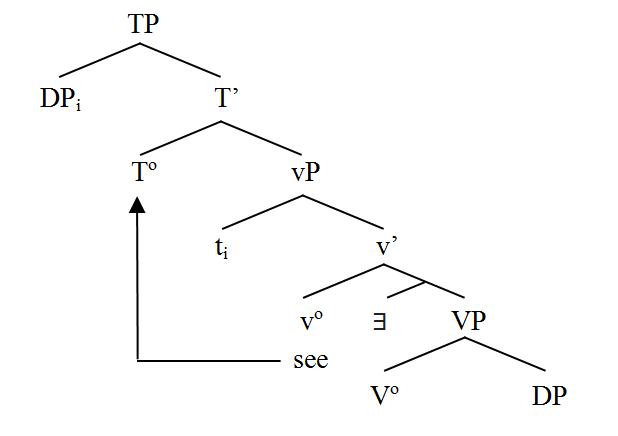
\includegraphics[width=\textwidth]{NgunaDuarteCamargotemplate-img1.png}
 \label{fig:1}
\end{figure}

  
\begin{figure}
%%please move the includegraphics inside the {figure} environment
%%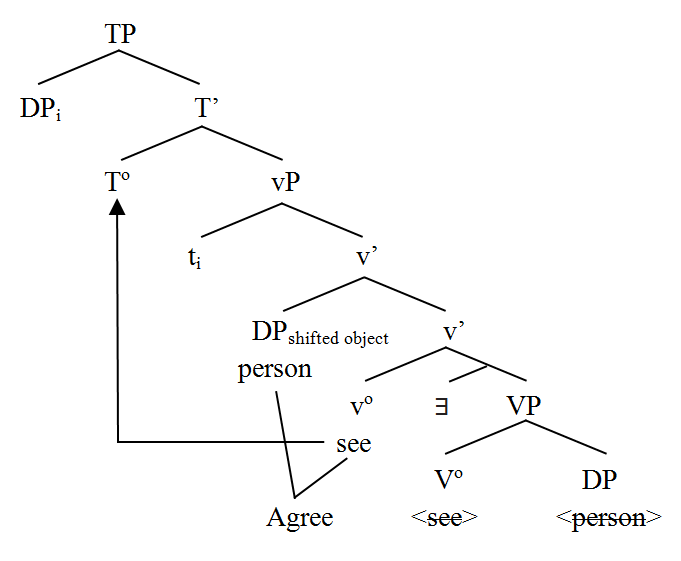
\includegraphics[width=\textwidth]{NgunaDuarteCamargotemplate-img2.png}
 

\caption{An object raised out of the VP allows a definite reading}
\label{fig:2}
\end{figure}

Given these background assumptions, we will assume, hereafter, that Rhonga and Changana set “yes” to Baker’s Directionality of Agreement Parameter (23). Notice that “F” can be read as the little \textit{v}\textsuperscript{o} that heads the {\textit{v}}P projection in \figref{fig:2}.

{The Directionality of Agreement Parameters \citep[155]{Baker2008}}

{\textit{F agrees with D/NP only if D/NP asymmetrically c-commands F.}}

This syntactic analysis entails that the head {\textit{v}} searches upward for the theme object to agree with, not downward. This accounts for why DP objects must move to Spec-{\textit{v}}P, or even to a higher position such as to a topic position.

\subsection{Arguments for the referential agreement analysis}

The data also provide evidence that the object prefixes behave more like referential agreement than pronoun incorporation, insofar as the object prefixes can co-occur with and match in person and number with the DP object in Emakhuwa, Shimakonde, Rhonga and Changana. All these languages allow a syntactic adjacency condition between the DP objects and the object prefixes in the transitive verb structure (though the DP need not occur in some discourse conditions, as in 17c) and (17e)), which must be interpreted as indicating that the DP object occurs in an internal argument position. This syntactic adjacency becomes apparent in the fact that DP objects that are referred to by the agreement prefix in the verbal complex are not prosodically separated from the verb, as would be expected if they were dislocated to an adjunct position. This syntactic co-occurrence possibility is taken here as evidence that the object prefixes are not incorporated pronouns, but are instances of referential agreement. This proposal is also in accordance with the assumption that pronominal inflection is clearly absent in languages that have agreement. In incorporated pronominal languages there is no DP inside the vP domain with which this inflection could agree \citep{Jelinek1989}. This is the case in languages like Egyptian Arabic, where pronominal inflections and DP objects are mutually exclusive \citep{Jelinek1989}, as is shown in (24).

{Egyptian Arabic}

\ea
\gll šuft-uh\\
     see-\textsc{3sg.m}\\
\glt ‘I saw him.’
\z

\ea
\gll šuft           il-walad\\
     see           the-boy\\
\glt ‘I saw the boy.’
\z

\citet{Jelinek1989} posits that the suffix -{\textit{uh}} does not function as agreement, but as an incorporated pronoun. She assumes that, as an incorporated pronoun occupies an argument position, it receives {a theta}{}-role in the usual way that core arguments of the verb do. The same pattern does not emerge in the Bantu languages examined here, since the object and the agreement prefix can co-occur without causing ungrammaticality, as data above show. Another piece of evidence that the Bantu object markers are really agreement in nature comes from the fact that they can only attach to the lower verb in contexts of verbal cluster constructions, as the Rhonga data in (25) indicate:

{Rhonga}

\ea
\gll mufana         a-gam-ile                ku-\textbf{xi}{}-b-a                   \textbf{xipixi}\\
     1.boy           1.\textsc{sm}{}-finish-\textsc{pst}        \textsc{inf}{}-7.\textsc{om}{}-hit-\textsc{fv}        7.cat\\
\glt ‘The boy finished hitting the dog.’
\z

\ea
\gll *mufana       a-\textbf{xi}{}-gam-ile                      ku-b-a            \textbf{xipixi}\\
     1.boy           \textsc{1.sm-7.om}{}-finish-\textsc{pst}         \textsc{inf}{}-hit-\textsc{fv}      7.cat\\
\glt (‘The boy finished hitting the dog.’)
\z

The fact that the object marker must occur in the embedded clause in (25) suggests that the lower verb must establish agreement first with the closest DP that is located in the little {\textit{v}}{\textsuperscript{o}} c-command domain. The fact that the object markers stay close to the lower verb is expected if they are agreement. If they were object clitics or incorporated pronouns, they would be able to attach to higher verbs in the structure. This proposal serves to reinforce the hypothesis that the object prefix is not an incorporated pronoun, but agreement, since there should be no object agreement on {\textit{v}} unless the agreed-with NP occurs in an argument position, that is, in the structural position of  Spec, {\textit{v}}P. Another piece of evidence in favor of this analysis comes from the fact that the object prefix cannot appear on the verb when it is in a passive voice, as in (26):

{Changana}

\ea
\gll ngonyama            yi-dlay-iw-ile               hi      muhloti\\
     9.lion                   9.\textsc{sm}{}-kill-\textsc{pass}{}-\textsc{pst}       by     1.hunter\\
\glt ‘The lion was killed (by the hunter).’
\z

\ea
\gll *ngonyama          yi-*\textbf{yi}{}-dlay-iw-ile                  hi       muhloti\\
     9.lion                   9.\textsc{sm-9.om}{}-kill-\textsc{pass-pst}       by      1.hunter\\
\glt (‘The lion was killed (by the hunter).’)
\z

The ungrammaticality of (26b) indicates that object agreement is sensitive to the locality condition and to the fact that the {\textit{v}}P must be in the active voice, and not in the passive one. In (26a) with a passive {\textit{v}}P, the DP object is raised from a position internal to the VP to the subject position, thereby blocking the occurrence of the object agreement prefix \{{\textit{yi}}{}-\}.

The next section is devoted to an analysis of DOM in double object constructions in Rhonga and Changana. The objective is to explain why the theme object, even when it is definite and specific, never triggers agreement in contexts where the verb selects two internal objects.

\subsection{Double Object Constructions}

{The d}ouble object constructions examined here all involve applicative constructions. {In general, }the literature proposes a distinction between \textit{symmetrical} and \textit{asymmetrical} object languages (Bresnan \& Moshi 1990; Chimbutane 2002; Ngonyani \& Githinji 2006). The two types of languages are diagnosed by syntactic tests involving: (a) object order, (b) passivization, (c) object marking and (d) relativization. In general, in Bantu languages it is observed that the \textsc{goal} or applied object (\textsc{ao}) can occur before the direct (\textsc{theme} or base) object (\textsc{do}) and vice-versa in symmetrical object languages, while the \textsc{goal} or applied object must precede the \textsc{theme} or base object in asymmetrical object Bantu languages. Only the \textsc{goal}/applied object may be passivized in asymmetrical object languages, whereas both can be passivized in symmetrical object languages. Furthermore, either object may trigger the object prefix on the verb stem in symmetrical object languages, as opposed to asymmetrical object languages in which only the goal may be cross-referenced on the verb. Based on these three tests, Bresnan and \citet{Moshi1990} propose the typology in \tabref{tab:3} to differentiate both types of (Bantu) languages.

%%please move \begin{table} just above \begin{tabular
\begin{table}
\caption{Bantu asymmetrical and symmetrical object languages}
\label{tab:3}


\begin{tabularx}{\textwidth}{XXX} & Symmetrical object Languages& Asymmetrical object languages\\
\lsptoprule
 Object order& {(i) AO DO}

 (ii) DO AO& (i) AO DO

 (ii) *DO AO\\
 Passivization& (i) AO

 (ii) DO& (i) AO

 (ii) *DO\\
 Object Marking& (i) AO

 (ii) DO& (i) AO

 (ii) *DO\\
\lspbottomrule
\end{tabularx}
\end{table}

In line with the assumptions above, {two questions must be addressed about the Rhonga and Changana}\footnote{ {We will not address the double object construction in Shimakonde and Emakhuwa owing to lack of enough empirical data. }} {applicative constructions, as follows: (i) Why does the verb never agree with the }{\textsc{theme}} {object, but only with the }{\textsc{goal}}{/}{\textsc{beneficiary}} {object? and (ii) Why is there just one agreement slot in the verbal morphological complex? }Our proposal is that Changana and Rhonga are asymmetrical object languages since \textsc{goal} arguments carry primary object properties, while \textsc{theme} arguments do not. This is confirmed by the following grammatical facts: (i) \textsc{goals} must precede \textsc{themes} in unmarked ditransitive sentences as in (27a); (ii) verb agreement must occur with the \textsc{goal} whenever it follows the \textsc{theme} object, as in (27b); (iii) only \textsc{goals} can be passivized, as in (27c). By unmarked ditransitive sentences, we refer to those syntactic contexts in which the \textsc{goal} is projected in a higher position than the \textsc{theme} object, thereby giving rise to the [Subject + Verb + \textsc{goal} + \textsc{theme}] word order.\footnote{ {According to \citet[111]{Chimbutane2002}, “there is consensus that in such cases the NPs immediately after the verb are mapped onto the thematically higher roles. This suggests, though not without controversy, that the position adjacent to the verb belongs to the arguments ranked thematically higher”.}} The bolding in (27) indicates the \textsc{goal}, be it in an (indirect) object (27a-b) position or in a subject (27c) position. Compare the examples below:

{Changana}

\ea
\gll nahani       a-svek-el-a                  \textbf{vapfumba}       tihlampfi\\
     1.aunt        1.\textsc{sm}{}-cook-\textsc{appl-fv}     2.guest            10.fish\\
\glt ‘My aunt is cooking fish for the guests.’
\z

\ea
\gll hahani       a-\textbf{va}{}-svek-el-a                       tihlampfi         \textbf{vapfumba}\\
     1.aunt        \textsc{1.sm-2.om}{}-cook-\textsc{appl}{}-\textsc{fv}     10.fish             2.guest\\
\glt ‘My aunt is cooking fish for them, the guests (and not chicken).’
\z

\ea
\gll \textbf{vapfumba}     va-svek-el-iw-a                       tihlampfi         (hi    hahani)\\
     2.guest          2.\textsc{sm-}cook-\textsc{appl-pass}{}-\textsc{fv}       10.fish              by    1.aunt\\
\glt ‘The guests are being cooked some fish (by my aunt).’
\z

{In example (27b), the object agreement prefix \{}{\textit{va-}}{\} refers to the }{\textsc{goal}} {object and emphasizes that it corresponds to given information in the discourse. Therefore the }{\textsc{goal}} {object must be interpreted as definite and specific in such construction. As the }{\textsc{theme}} {object carries new information in (27b), it must move around the }{\textsc{goal}} {object to a dedicated focus position in the left periphery of the }{\textit{v}}{P}{\textit{. }}{Evidence that the }{\textsc{theme}} {object really represents the contrastive focus comes from the fact that sentence (27b) denotes the semantic interpretation that ‘my aunt is cooking fish and not chicken for the guests’. This grammatical pattern is confirmed by the fact that the sentence becomes ungrammatical if the agreement prefix \{}{\textit{va}}{{}-\} occurs on the verb stem and the }{\textsc{goal}} {object remains in its unmarked (i.e. immediately postverbal) position, thereby occupying a syntactic position before the }{\textsc{theme}} {object, as }in (28):

{Changana}

\ea
\gll *{hahani       a-}{\textbf{va}}{{}-svek-el-a                        }{\textbf{vapfumba}}         {tihlampfi}\\
     1.aunt          1.{\textsc{sm}}{{}-2.}{\textsc{om}}{{}-}cook{{}-}{\textsc{appl}}{{}-}{\textsc{fv}}       {}2.guest             {10.}fish\\
\glt (*‘My aunt is cooking fish for them, the guests.’)
\z



Based on the fact that the \textsc{goal} (i) is generated in a high thematic position; (ii) controls object agreement; and (iii) is subject to passivization, one possibility is to posit that the \textsc{goal} argument is then introduced in a high syntactic position, while the \textsc{theme} object is generated in a low syntactic position. Let’s then propose that the \textsc{goal} object is first merged as a specifier of a high Applicative Phrase (ApplP), which allows it to be base-generated between the \textsc{agent} and the \textsc{theme} objects, as depicted in \figref{fig:3}.

  
%%please move the includegraphics inside the {figure} environment
%%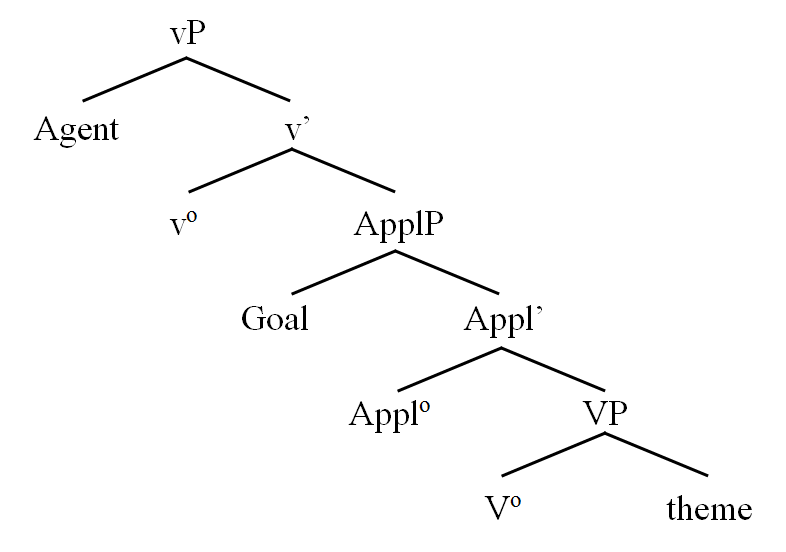
\includegraphics[width=\textwidth]{NgunaDuarteCamargotemplate-img3.png}
 

\begin{figure}
\caption{Double object construction structure in Changana}
\label{fig:3}
\end{figure}

In double object constructions, at least in {asymmetrical object languages such as Rhonga and Changana,}\footnote{ {We refer the reader to Chimbutane’s (2002) arguments for Changana as an asymmetrical object language.}} {}the \textsc{theme} object is never cross-referenced on the verb. Let’s then assume that the agreement between the \textsc{goal} and the little {\textit{v}} takes place at the moment when the lexical verb performs successive cyclic movement from V-to-Appl and then from Appl-to-{\textit{v}}. Additionally, let’s postulate that this head movement operation is followed by the \textsc{goal} object shift from the specifier of ApplP to the specifier of {\textit{v}}P. Under this view, the agreement between the applied object and the verb follows from the Directionality of Agreement Parameter, proposed in (23), according to which a head F (i.e. the little light verb) agrees with a DP only if that DP asymmetrically c-commands F. This proposal has the advantage of accounting for why only the applied (=\textsc{goal/beneficiary}) argument controls the agreement on the verb complex, whereas the \textsc{theme} argument cannot. In short, this analysis presupposes that both the verb and the applied object are in the same local domain at the moment that the agree operation takes place. The derivation proposed here entails that the sentence in (29) has the syntactic derivation shown in \figref{fig:4}. In this derivation, moving the \textsc{theme} object around the \textsc{goal} to Spec-{\textit{v}}P would put it before the \textsc{goal} object and the verb, thereby yielding [\textsc{theme-goal}{}-Verb] word order. A way to restore the superficial [Verb-\textsc{theme-goal}] word order is to propose that the verb subsequently moves to the {\textsc{infl}} node (Tense/Aspect/Mood domain) of the clause, as depicted by the derivation in \figref{fig:4}.

\ea
{Changana}

\gll hahani       a-va-svek-el-a                        tihlampfi      vapfumba\\
     1.aunt        1.{\textsc{sm}}{{}-2.}{\textsc{om}}{{}-}cook{{}-}{\textsc{appl}}{{}-}{\textsc{fv}}      {10.}fish          2.guest\\
\glt ‘My aunt is cooking fish for them, the guests.’
\z

 
\begin{figure}
%%please move the includegraphics inside the {figure} environment
%%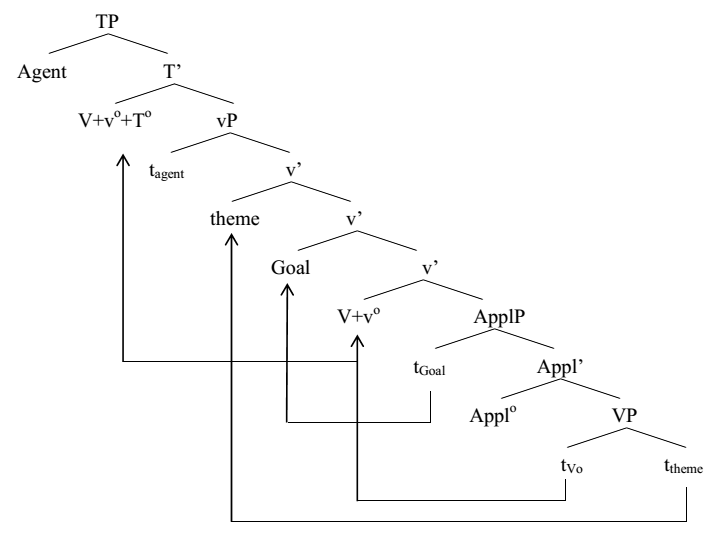
\includegraphics[width=\textwidth]{NgunaDuarteCamargotemplate-img4.png}

\caption{Syntactic derivation of the [{\textbf{\textsc{subject+verb+theme+goal]}}} word order}
\label{fig:4}
\end{figure}

An immediate consequence of the syntactic derivation outlined here is that it reinforces the proposal advanced in §4.1, according to which the object prefix is not an incorporated pronoun, but simply referential agreement. Evidence comes from the fact that the verb agrees only with the \textsc{goal} object, which must be positioned internal to the {\textit{v}}P domain and not dislocated to a right or left-peripheral position. Additionally, the fact that the DP \textsc{goal} occurs inside the vP/ApplP domain corresponds to it not being in an adjunction position, but in an argument position. Recall that in incorporated pronoun languages, the DP object and the pronominal inflection cannot co-occur in the same domain, since they are in complementary distribution. In conclusion, as the data above show, such distribution does not occur in the Bantu languages examined here, since the DP object, regardless of whether it is \textsc{goal} or \textsc{theme}, must remain within domain of the {\textit{v}}P for the verb to establish agreement with it.

\section{Final remarks}

In this paper, we have shown that object agreement in Emakhuwa can be interpreted as the realization of a noun class hierarchy, whereas in Shimakonde it is regulated by the animacy and definiteness hierarchy: human {\textgreater} definite animate {\textgreater} inanimate, with definite animate and human nouns controlling object agreement in the verbal complex. Object marking in Changana and Rhonga is regulated not by animacy, but only by definiteness and specificity. Only specific and definite DPs can trigger object agreement in simple transitive predicates.

Regarding double object constructions, the analysis has shown that there is just one slot per clause for object agreement. We have proposed that what regulates the occurrence of agreement in this context is locality, with the \textsc{goal} object merging in a higher position than the \textsc{theme} object in the syntactic structure. This means that \textsc{goal} object is the closest candidate for the little {\textit{v}} head to agree with. This in turn accounts for why agreement with \textsc{theme} object is systematically forbidden in the double object constructions. 

We have also presented empirical evidence in favor of the analysis that the object prefixes behave more like referential agreement than pronoun incorporation, namely: (i) object prefixes match in person and number with the DP object in Shimakonde, Rhonga and Changana; (ii) in these languages, the DP object that triggers the object prefix on the verb stem must appear within the \textit{v}P, which is reflected in the fact that the object is not prosodically separated from the verb. The only exception is Emakhuwa where animacy/humanness over-rides class/gender. These facts lead one to assume the DP object sits in an internal specifier position of \textit{v}P. This then reinforces the hypothesis that the \textsc{theme} object remains in a nuclear position within the v-VP and not in an adjunction position.

\section {Abbreviations}

{\textsc{1  }}{first person}

{\textsc{2  }}{second person}

{\textsc{3  }}{third person}

{\textsc{acc  }}{accusative}

{\textsc{ao  }}applied object

{\textsc{appl  }}{applicative}

{\textsc{cont}}  {contactive}

{\textsc{def  }}{definite}

{\textsc{do  }}direct object

\textsc{dom}  double object marking

{\textsc{fv  }}final vowel

{\textsc{inf  }}infinitive

{\textsc{loc}}  locative

{\textsc{m  }}masculine

{\textsc{om  }}object marker

{\textsc{part  }}particle

{\textsc{pass  }}passive

{\textsc{pl  }}plural

{\textsc{prf  }}perfective

{\textsc{pst  }}past

{\textsc{rel}}  relative marker

{\textsc{sg  }}singular

{\textsc{sm  }}subject marker

{\textsc{t}}/{\textsc{a  }}tense and aspect marker

\section {References}

\begin{verbatim}%%move bib entries to  localbibliography.bib

Croft, William. 1988. Agreement vs. case marking and direct objects. In Barlow, Michael & Ferguson, Charles (eds.), Agreement in natural language: Approaches, theories, descriptions. Chicago: University of Chicago Press.

Downing, Laura. 2014. Differential object marking in Chichewa. (Paper presented at the workshop of The Diachronic Typology of Differential Argument marking, University of Konstanz, April 5-6, 2014.)



Givón, Talmy. 1976. Topic, pronoun and grammatical agreement. In Li, Charles (ed.), Subject and Topic. New York: Academic Press.

Jelinek, Eloise. 1989. The case split and pronominal arguments in Choctaw. In Maracz, La\' szló & Muysken, Pieter (eds.), Configurationality: The typology of asymmetries. Dordrecht: Foris Publications.




Woolford, Ellen. 2001. Conditions on object Agreement in Ruwund (Bantu). In Benedicto, Elena (ed.), The UMass volume on indigenous languages. Amherst: GLSA.




\end{verbatim}

\section*{Abbreviations}
\section*{Acknowledgements}

\printbibliography[heading=subbibliography,notkeyword=this]

\end{document}